\chapter{Beyond the training horizon}
\begin{quotation}
\noindent ``\emph{quote}''
\begin{flushright}\textbf{author}\end{flushright}
\end{quotation}


So far, we have tested our agent only within the limits of what it has been
trained. What happens if we leave it running for more episodes than what it
has been trained for?

\section{Testing performance after the training horizon}
We have trained an agent on the 20 permutations listed in
Table~\ref{tab:20perms}a, with inverted actions, over trials of 5 episodes.
We can test the agent on trials of more episodes - meaning that the hidden
state will be carried on until the end of the 20th episode.
Figure~\ref{fig:horizon_5_20} shows the result of this experiment.\\

\begin{figure}
	\centering
	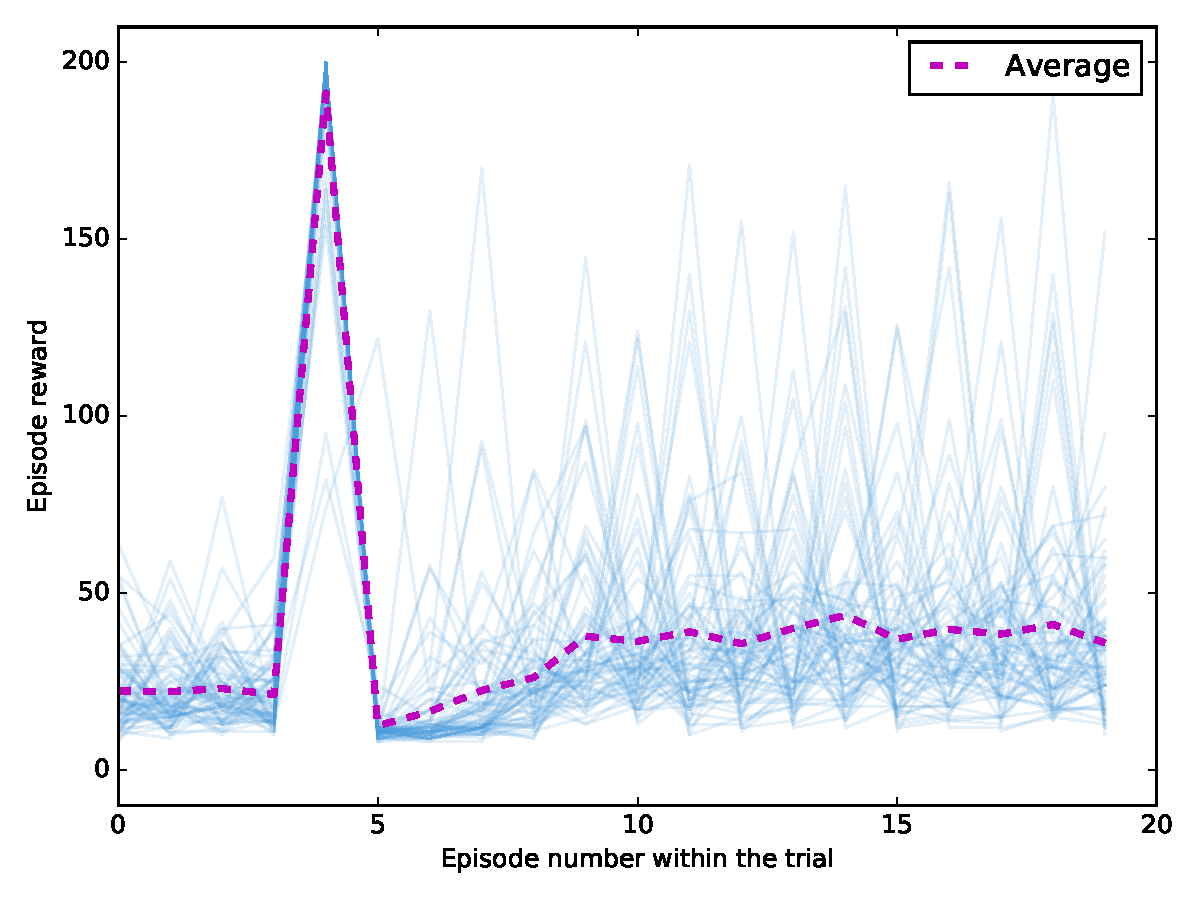
\includegraphics[width=0.8\linewidth]{fig/horizon_5_20.pdf}
	\caption{Testing performance over 20 episodes of an agent trained on 
	trials of 5 episodes only. Several runs are shown in blue, their
	average is plotted in red dashes.}
	\label{fig:horizon_5_20}
\end{figure}

There is no surprise in the rewards obtained for episodes 0 to 4. The pattern
observed from episode 5 onwards, however, deserve commenting. The lowest
average episode reward stands at episode 5 (the first episode beyond the
training horizon); then the average rewards climbs slowly to reach a baseline
level which is higher than the one prior to the optimal episode. This leads us
to believe that training on trials that contain more episodes could lead to 
better reward after the training horizon.

\subsection{Restoring recurrent weights}
One solution to maintain a high reward after the training horizon would be 
to restore the recurrent weights to their state prior to the last episode of 
the training horizon at the beginning of each episode. As 
Figure~\ref{fig:horizon_5_20_restoring} shows, this solution works.\\

\begin{figure}
	\centering
	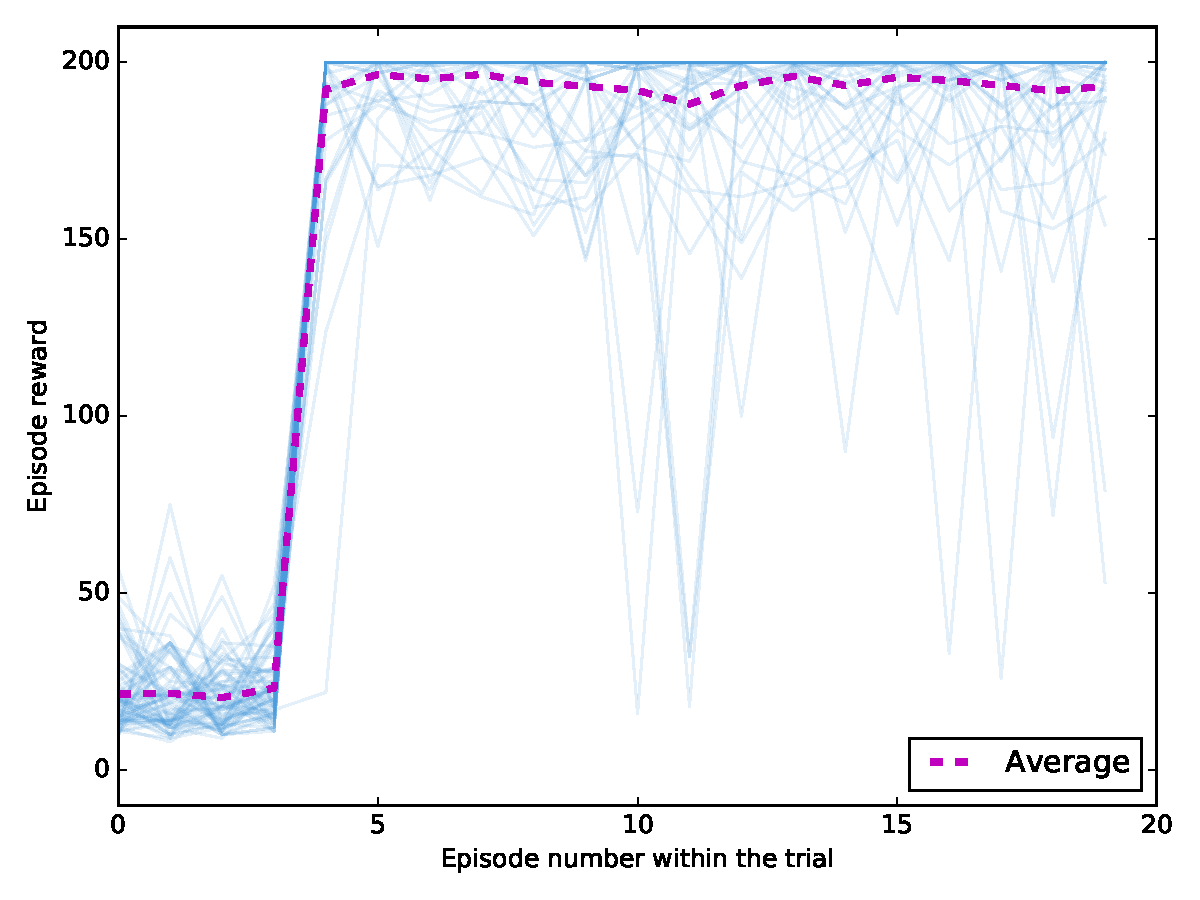
\includegraphics[width=0.8\linewidth]{fig/horizon_5_20_restoring.pdf}
	\caption{Testing performance over 20 episodes of an agent trained on 
	trials of 5 episodes only. The recurrent weights are saved prior to 
	the 5th episode and restored prior to each episode from the 6th episode
	onwards. Several runs are shown in blue, their average is plotted in
	red dashes.}
	\label{fig:horizon_5_20_restoring}
\end{figure}

This result is not a surprise, and this solution should rather be called a 
workaround. Indeed, restoring the weights at the beginning of each episode
stops any learning to occur after the preset training horizon. Although the
agent is supposed to have reached an optimal policy at the end of the training
horizon, we cannot assume there is nothing left to learn as the agent navigates
through later episodes.

\section{Training on more episodes}

\begin{figure}
	\centering
	\includegraphics[width=0.8\linewidth]{fig/horizon_10_20_restoring.pdf}
	\caption{Testing performance over 20 episodes of an agent trained on 
	trials of 10 episodes only. 
	Several runs are shown in blue, their average is plotted in red dashes.}
	\label{fig:horizon_10_20}
\end{figure}
